\chapter{The \ui{FxmeNet} plugin}
\label{ch:plugin}

This chapter walks through the plugin's window, then explains how it works
with the DAW: automation, saving projects, bypass and latency.

\section{The window}

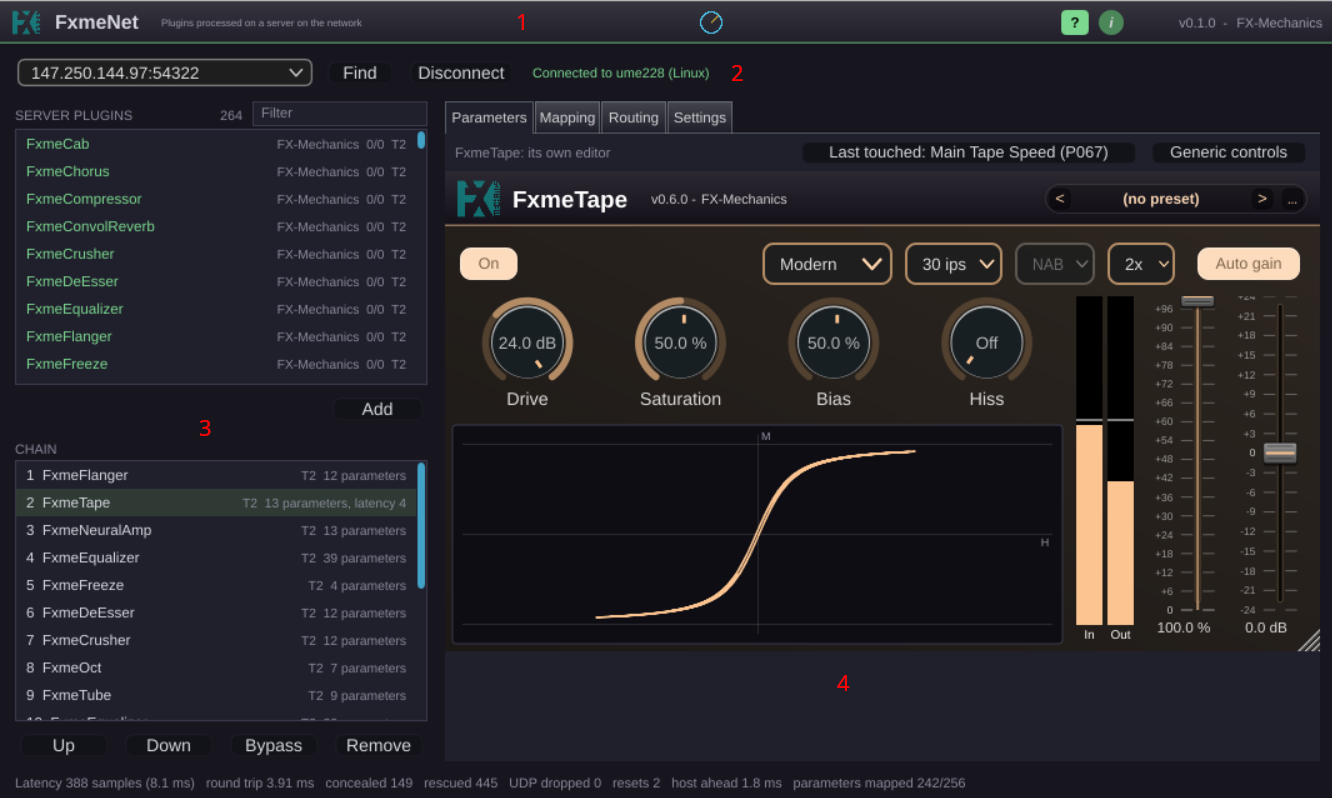
\includegraphics[width=\textwidth]{../img/fxme-net-plugin-screen.png}

From top to bottom:

\begin{description}
  \item[Top bar.] The FX-Mechanics logo and version, a \ui{?} switch that
    turns the hover help on or off for all instances, and an information
    button.
  \item[Server row.] The server's address, \ui{Find} and \ui{Connect} (the
    button reads \ui{Disconnect} while connected), and the connection
    status.
  \item[Left column.] \ui{SERVER PLUGINS}, the list of what the server offers,
    with its filter and the \ui{Add} button; and \ui{CHAIN}, your plugins
    in processing order, with \ui{Up}, \ui{Down}, \ui{Bypass} and
    \ui{Remove}.
  \item[Right side.] Four tabs: \ui{Parameters}, \ui{Mapping}, \ui{Routing}
    and \ui{Settings}.
  \item[Bottom line.] Statistics (section~\ref{sec:stats}).
\end{description}

\section{Connecting}

Type the server's address (a name or an IP address, with \cmd{:port} if it
does not use the default) or press \ui{Find} and choose a server from the
list that appears. \ui{Connect} opens the session. While the plugin is not
connected, the audio passes through untouched. The plugin remembers the last
server you used, on this computer, and connects again when you reopen a
project.

If the connection drops, the plugin reconnects by itself and resumes its
session when the server still has it (section~\ref{sec:sessions}).

\section{Choosing plugins}

\ui{SERVER PLUGINS} lists what the server offers. Each row shows the plugin's
name, its vendor, its input and output channels, and a tag \tier{2},
\tier{1} or \tier{0} that says how the plugin can be shown on this computer
(chapter~\ref{ch:tiers}). Hover over a row to see why it has its tier.

The list is sorted by tier (\tier{2} first, then \tier{1}, then \tier{0}) and
by name inside each tier. While the plugin scans this computer for the first
time, the order is by name only, and the tags read \tier{?}.

To find a plugin quickly, type a few letters in the \ui{Filter} field above
the list. Only plugins whose name contains every word you type remain. The
first match is selected: press \key{Return} to add it. \key{Esc} clears the
filter. \ui{Add} (or a double-click) adds the selected plugin at the end of
the chain.

\section{The chain}

\ui{CHAIN} lists your plugins in the order the server processes them, from
top to bottom. Select one to see its controls on the right. Buttons under
the list:

\begin{description}
  \item[Up, Down] Move the selected plugin in the chain.
  \item[Bypass] Bypass the selected plugin, on the server.
  \item[Remove] Remove it. The state of the plugin is lost.
\end{description}

A plugin that cannot be loaded on the server shows the reason in red (a
missing licence, a plugin that failed to start, ...).

The routing between the plugins is serial by default, as in a plain chain. To
do parallel processing or sidechains, see chapter~\ref{ch:routing}.

\section{The Parameters tab}

The tab shows the selected plugin.

\begin{itemize}
  \item If the plugin is installed on this computer in the same version
    (tier \tier{1} or \tier{2}), you see its own editor. It is a local copy,
    kept in step with the server: what you change in it is sent to the
    server, and what changes on the server appears in it. The window grows
    to fit the editor and returns to its normal size when you leave it.
  \item Otherwise, you see generic controls: one row per parameter with its
    name, a slider and its value. Double-click a slider to return to the
    default.
\end{itemize}

A button above the controls switches between the plugin's own editor and the
generic controls. A \ui{last touched} button next to it names the control you
moved last in the plugin's editor, with a menu to map it to an automation
parameter (below).

\section{Automation}

The DAW sees \fxme\ as one plugin with 256 automation parameters, named
\texttt{p001} to \texttt{p256} until they are used. When a plugin joins the
chain, its automatable parameters take the first free entries, and the DAW
shows them under the plugin's name (for example ``FxmeCompressor: Ratio'').
You can automate them, and the DAW's own controls, as with any plugin.

The \ui{Mapping} tab lists every entry in use and what it controls. To free
entries, select them and press \ui{Unmap}, or use \ui{Unmap all}.

To map a parameter by hand, use one of the two methods:

\begin{itemize}
  \item In the generic controls, press \ui{Map} on a row to give it the first
    free entry.
  \item Press \ui{Learn}, then move any of \fxme's parameters in the DAW: the
    parameter you moved becomes the one that controls it.
\end{itemize}

\begin{note}
Automation lanes in the DAW belong to the numbered entries. When you remove a
plugin, its entries stay free but keep their lane. \fxme\ does not give a
used entry to the next plugin you add (unless you map it by hand or all 256
have been used), so a recorded automation cannot silently drive another
plugin's parameter.
\end{note}

\section{Settings}

The \ui{Settings} tab has three parts.

\begin{description}
  \item[Stream.] \ui{Block size N} and \ui{Network budget D}, with the latency
    they give (chapter~\ref{ch:performance}).
  \item[Transport.] \ui{Silence in-flight audio at reset}: when the DAW restarts
    playback or jumps, drop the audio still on its way back from the server,
    so you hear silence for the length of the latency (as a local plugin
    clearing its delay line) rather than the tail of the previous position.
    \ui{Log transport events} writes what the audio thread sees around
    transport events, concealed blocks included, to
    \file{fxmenet-client-events.log} in the FX-Mechanics settings folder; it
    is for diagnosing problems.
  \item[Local plugins.] The scan of the plugins installed on \emph{this}
    computer, used for the plugins' own editors. \ui{Rescan} looks for new or
    changed plugins; \ui{Full rescan} examines everything again;
    \ui{Folders\ldots} adds folders to search beside the standard VST3 ones.
\end{description}

\section{Statistics}
\label{sec:stats}

The line at the bottom of the window gives:

\begin{description}
  \item[Latency] What \fxme\ reports to the DAW, in samples and milliseconds.
  \item[Round trip] The last measured time for a message to reach the server
    and come back.
  \item[Concealed] Blocks that came back too late and were replaced.
  \item[Rescued] Blocks that would have been concealed but arrived in time
    after a short wait.
  \item[UDP dropped] Audio messages the client threw away because they could not be put together: pieces missing, damaged or too large. It should stay at zero on a healthy network.
  \item[Resets] How many times the DAW reset the plugin (playback start, stop or a jump in the timeline). Each time, the server resets its chain at the same point of the stream.
  \item[Host ahead] How far the DAW processes audio ahead of real time, in milliseconds. It is 0 when the DAW calls the plugin at the pace of the sound card, and larger when the DAW renders with a read-ahead buffer.
  \item[Parameters mapped] How many of the 256 entries are in use.
\end{description}

A concealed count that rises steadily means the server or the network cannot
keep up with the chosen settings (chapter~\ref{ch:performance}).

\section{Bypass, projects and offline rendering}

\begin{itemize}
  \item \textbf{DAW bypass.} When you bypass \ui{FxmeNet} in the DAW, the
    plugin passes the audio dry, delayed by the same latency, so that
    switching it on and off does not move the track in time.
  \item \textbf{Saving.} The project stores the server, the settings, each
    plugin with its state, the parameter mapping and the routing. When you open
    the project, the plugin rebuilds the chain on the server and connects. If
    the server is not reachable then, the plugin keeps the state, and you can
    connect later.
  \item \textbf{Offline rendering.} When the DAW renders faster than real
    time (a bounce or an export), the plugin waits for each reply, so
    nothing is concealed and the result is exact.
\end{itemize}

\section{The same project on another computer}
\label{sec:sessions}

A project that uses \fxme\ needs the server to be reachable and to have the
same plugins installed. If a plugin is missing on the server, its row in the
chain shows an error and the audio is not processed by it. The audio goes through that position of the chain unchanged, as if the plugin were bypassed, and the rest of the chain keeps working. A future release will let you optionally compute the chain locally on the client when the server is not available.
